\documentclass[mathserif, handout]{beamer}
\usetheme{CambridgeUS}
\definecolor{USCred}{rgb}{0.6,0,0}
\usecolortheme[RGB={153,0,0}]{structure}
\useinnertheme{circles}
\setbeamertemplate{navigation symbols}{}
\usepackage{bm}
%\usepackage{subfig}
%\usepackage{algorithmic}
\usepackage[square]{natbib}
\usepackage{amsmath}
\usepackage{amssypmb}
\usepackage{graphicx}
\usepackage{soul}
\usepackage{caption}
\usepackage{subcaption}
\usepackage{verbatim}
\usepackage{algorithmic}
\usefonttheme[onlymath]{serif}

%\usepackage[numbered]{algo}
%
% \AtBeginSection[]
% {
%   \begin{frame}
%     \frametitle{Table of Contents}
%     \tableofcontents[currentsection]
%   \end{frame}
% }

\title[Fall 2014]{Fall 2014}
\institute[USC]{
  University of Southern California
}

\begin{document}

\maketitle
%%%%%%%%%%%%%%%%%%%%%%%%%%%%%%%%%  Slide 0  %%%%%%%%%%%%%%%%%%%%%%%%%%%%%%%%%%%%%%%%%%%
\begin{frame}{Summary}

\begin{itemize}
\item TA for Machine Learning (50\%)
\item Two classes
\item Meeting...meetings...
\item Submitted one paper with Max
\item Research project with Fei (collaboration with Yuan)
\item Research project with Yan
\end{itemize}
\end{frame}



\begin{frame}{Scalable inference for overlapping communities}
\begin{figure}
  \begin{subfigure}[b]{.2\linewidth}
    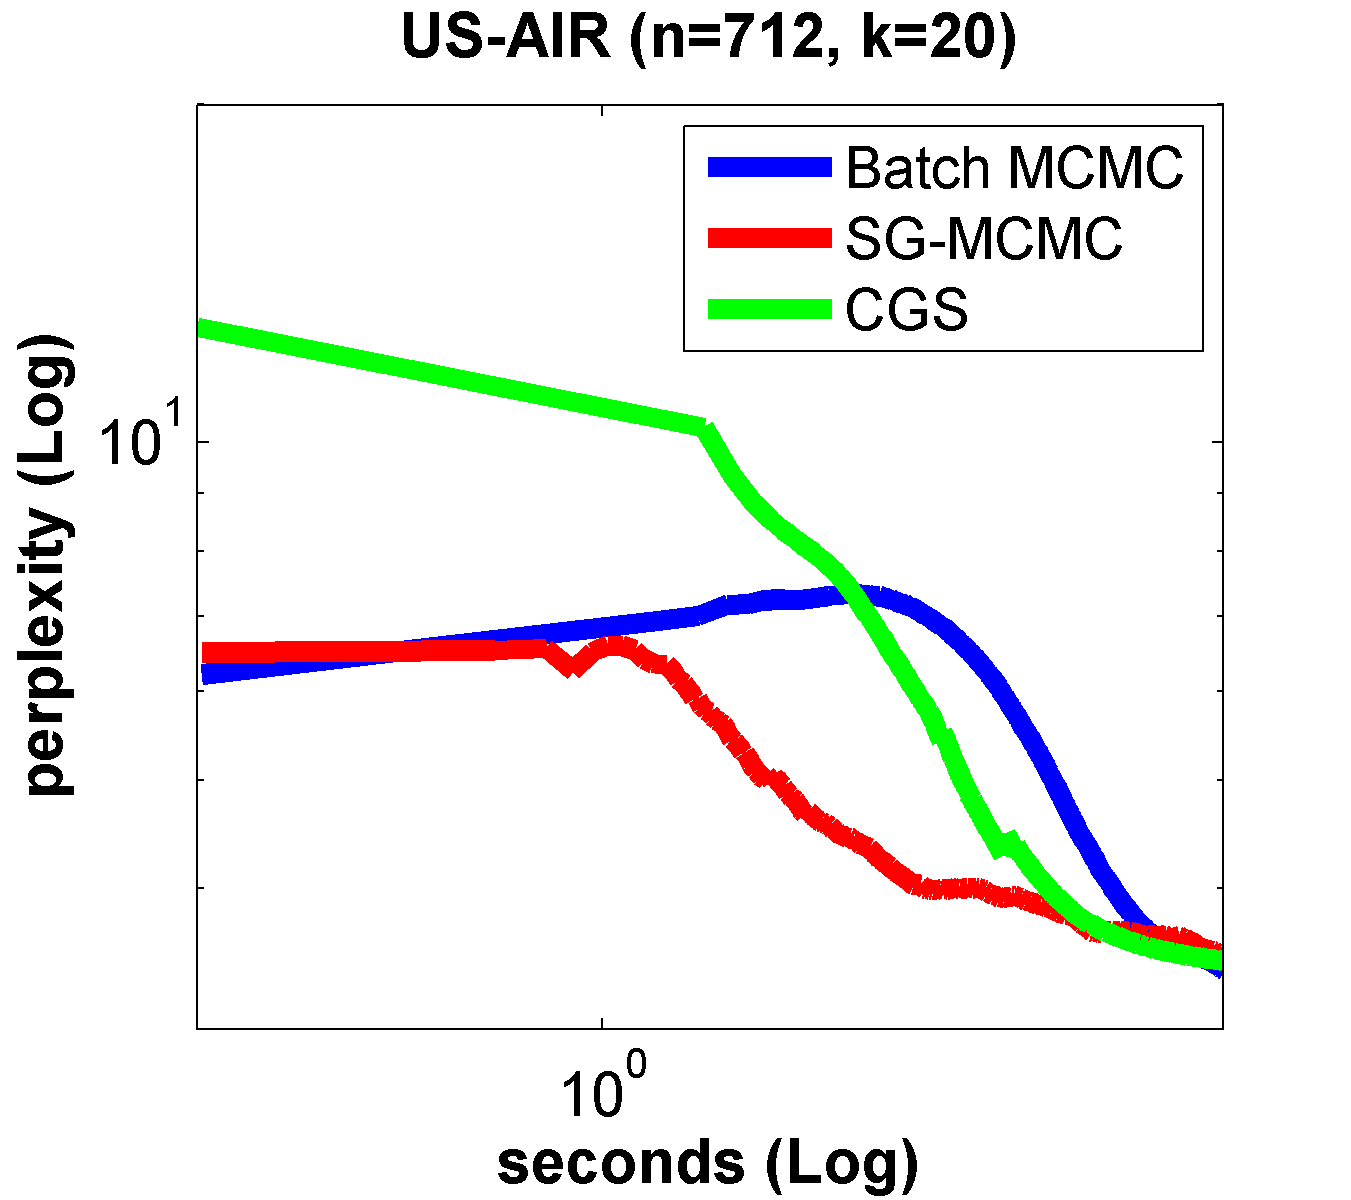
\includegraphics[height=2cm]{1st_usair.png}
  \end{subfigure}
  \begin{subfigure}[b]{.2\linewidth}
    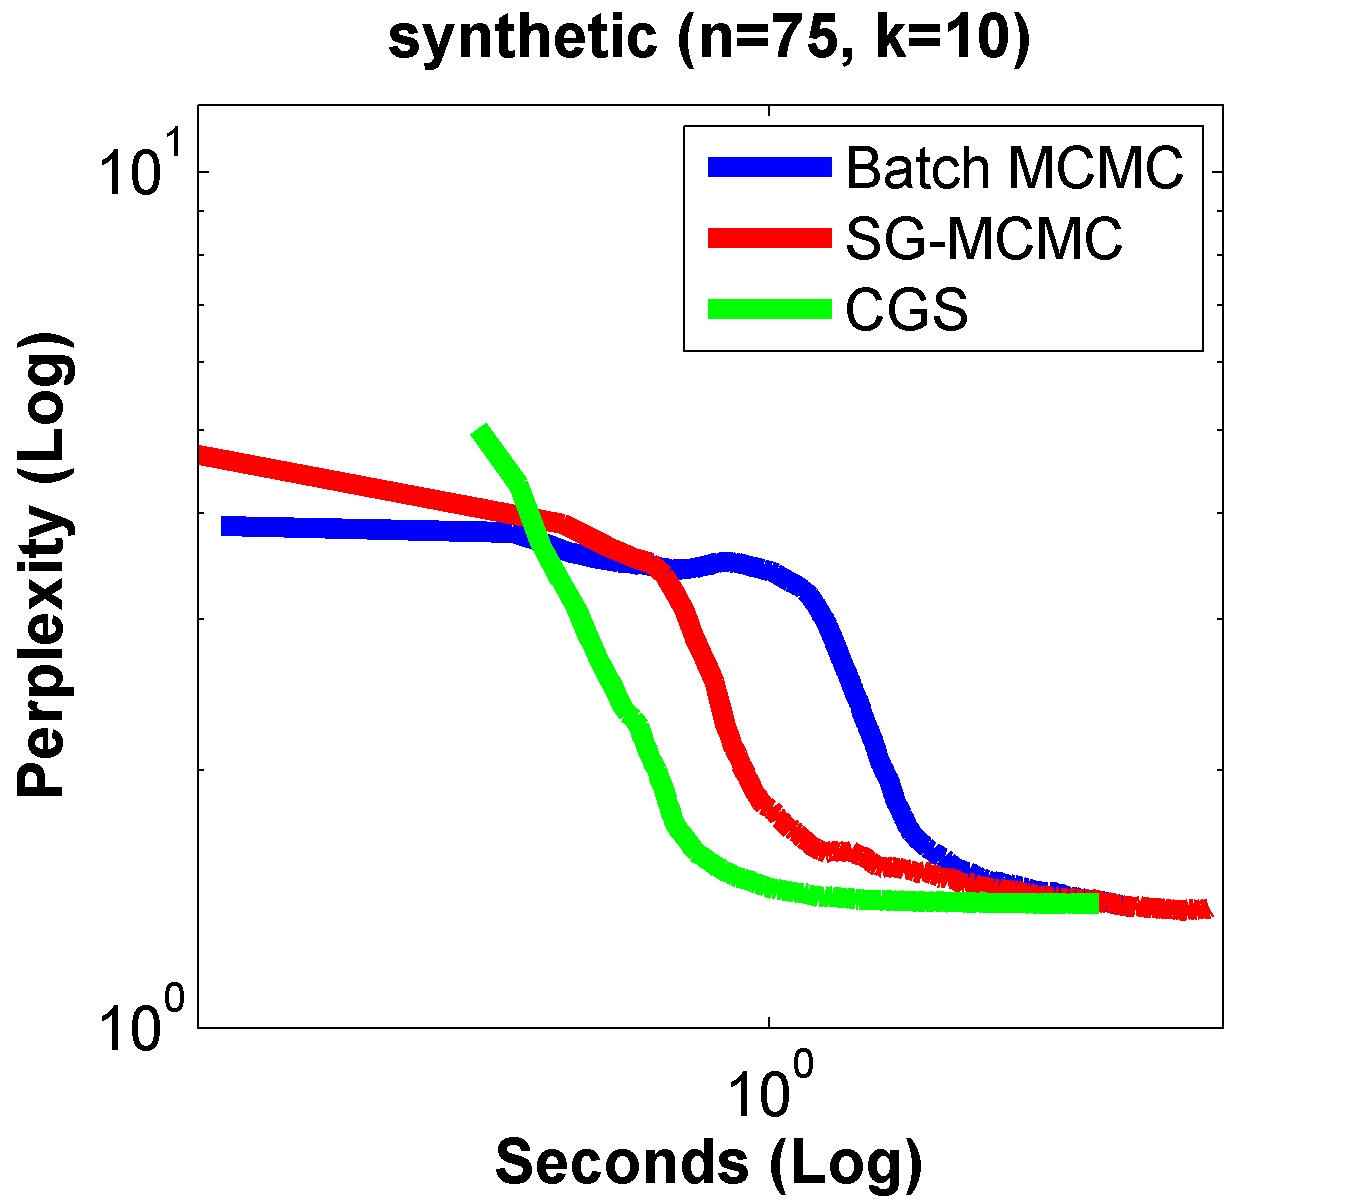
\includegraphics[height=2cm]{compare_1.png}
  \end{subfigure}\\
\caption{Batch MCMC vs SG-MCMC vs CGS}\label{fig:1}
\end{figure}


\begin{figure}
  \begin{subfigure}[b]{.2\linewidth}
    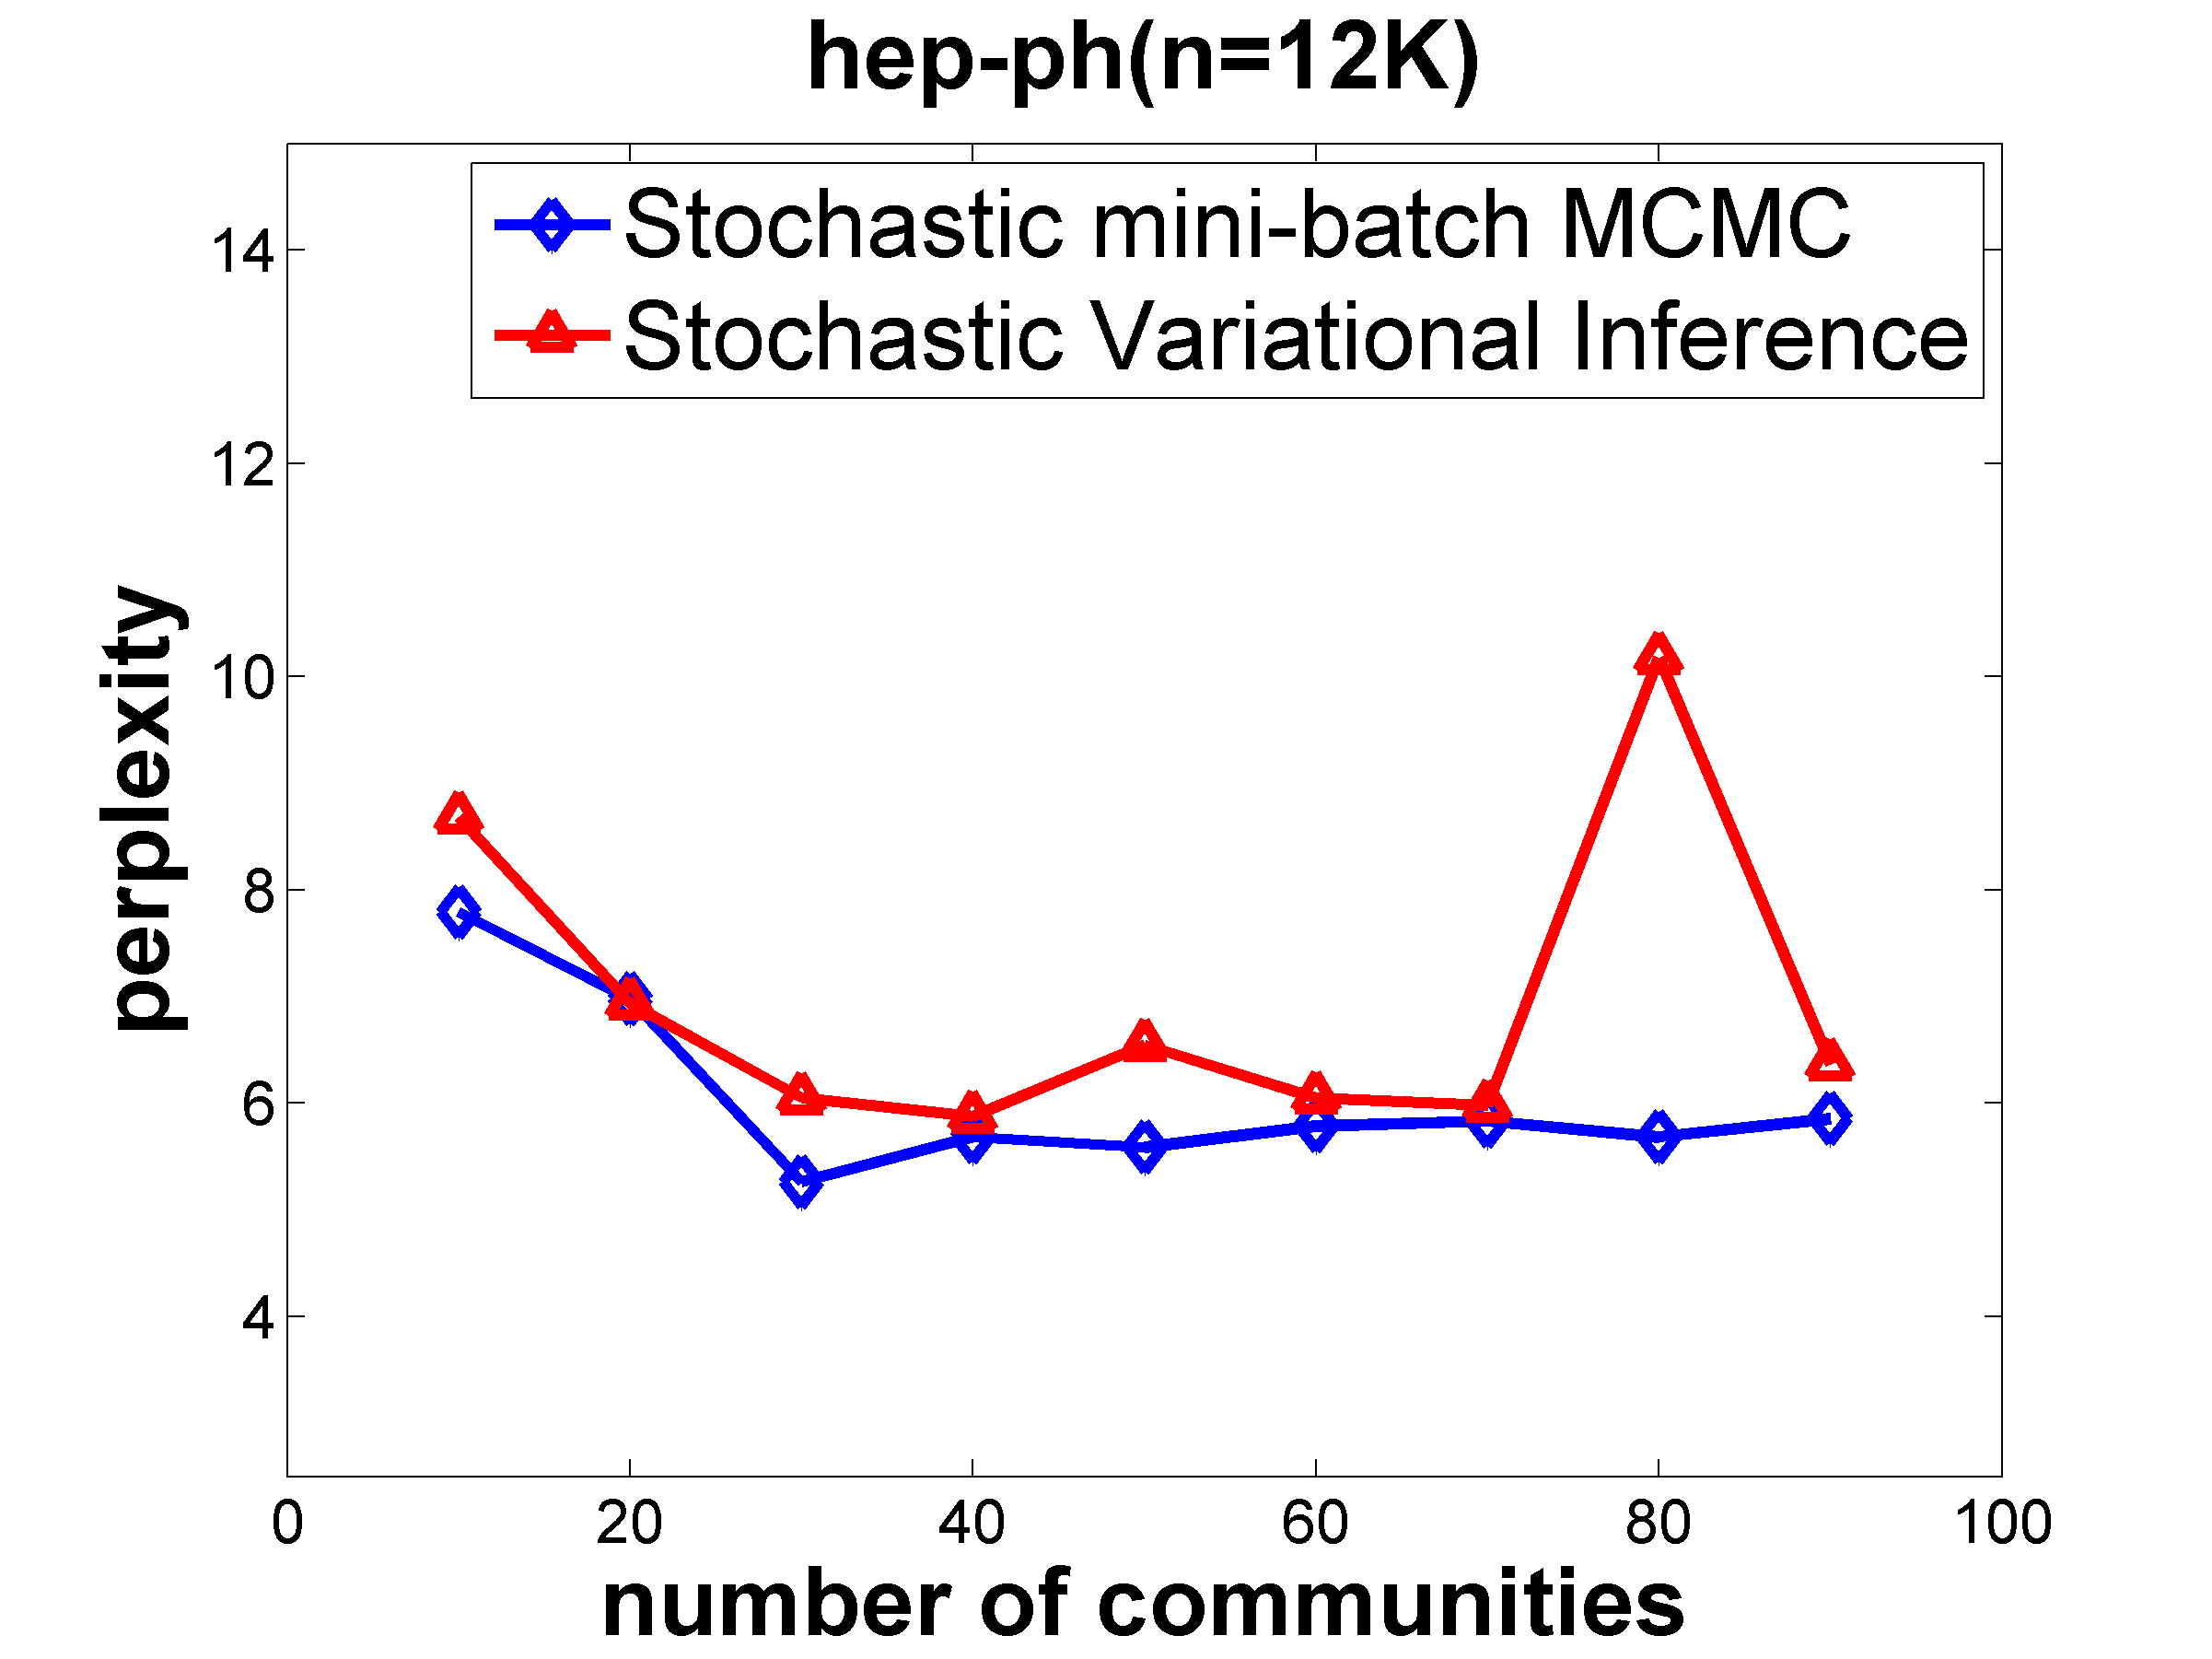
\includegraphics[height=2cm]{3rd_hepph}
  \end{subfigure}
  \begin{subfigure}[b]{.2\linewidth}
    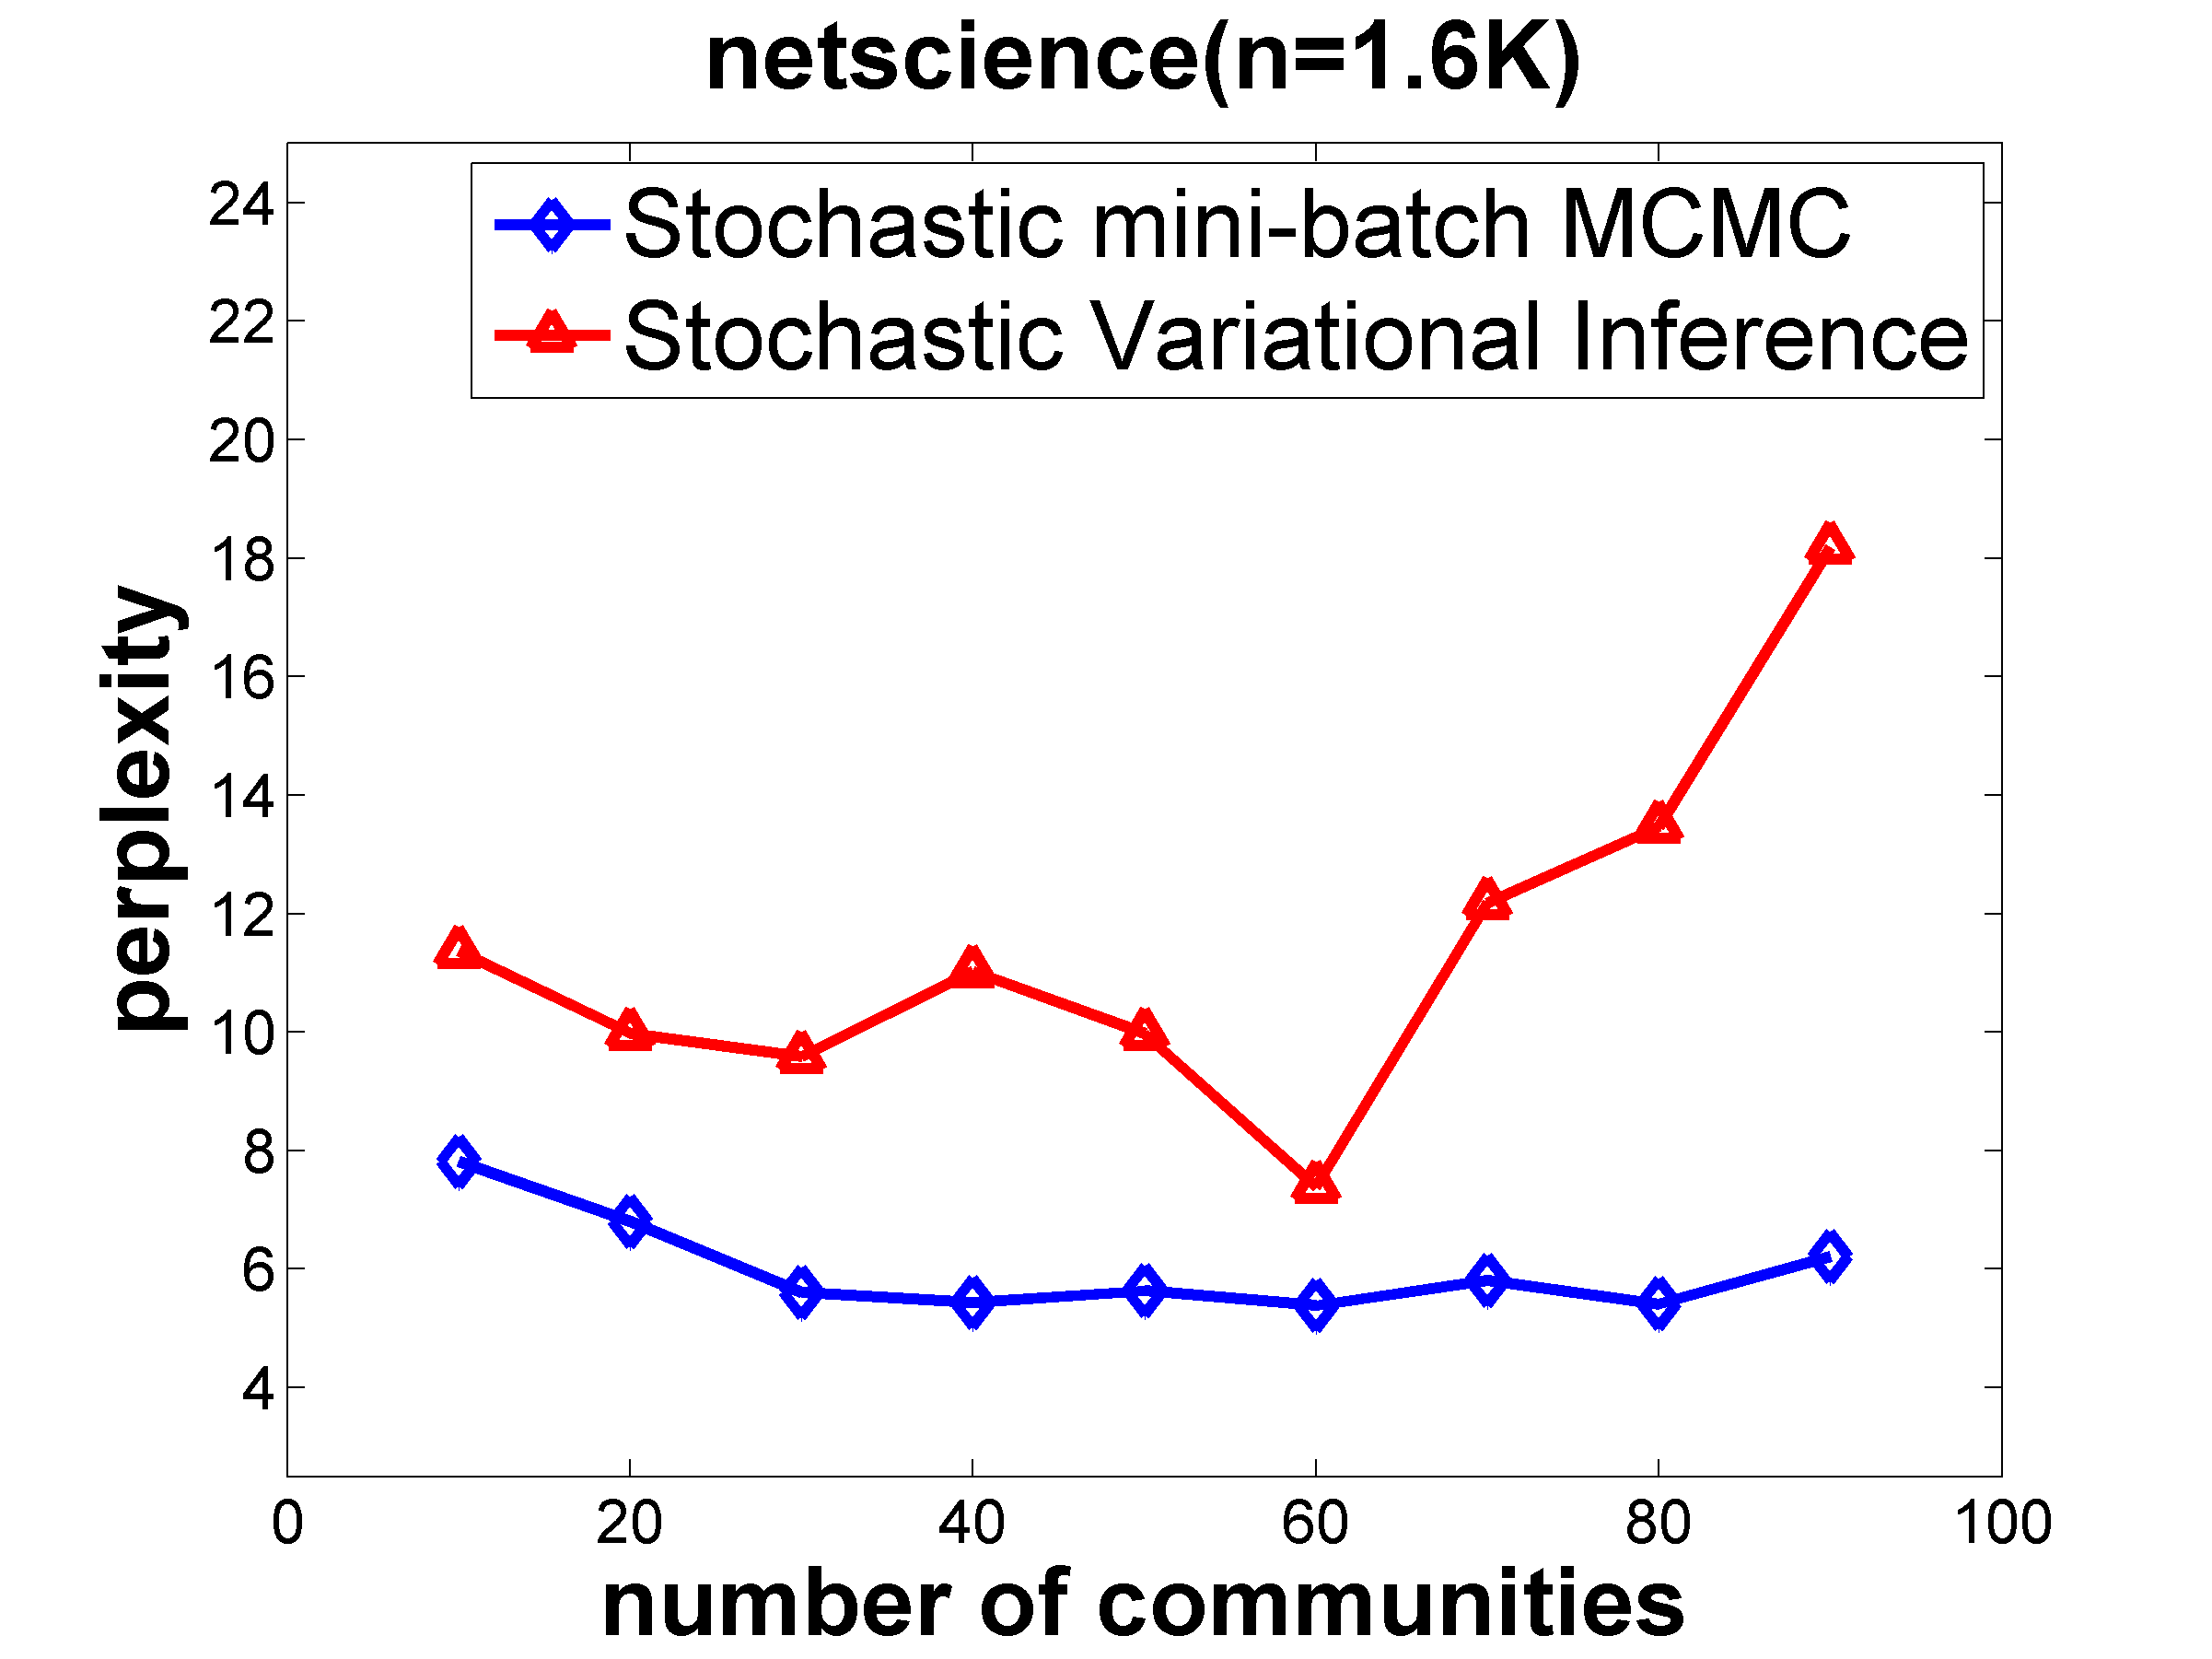
\includegraphics[height=2cm]{3rd_netscience}
  \end{subfigure}
  \begin{subfigure}[b]{.2\linewidth}
    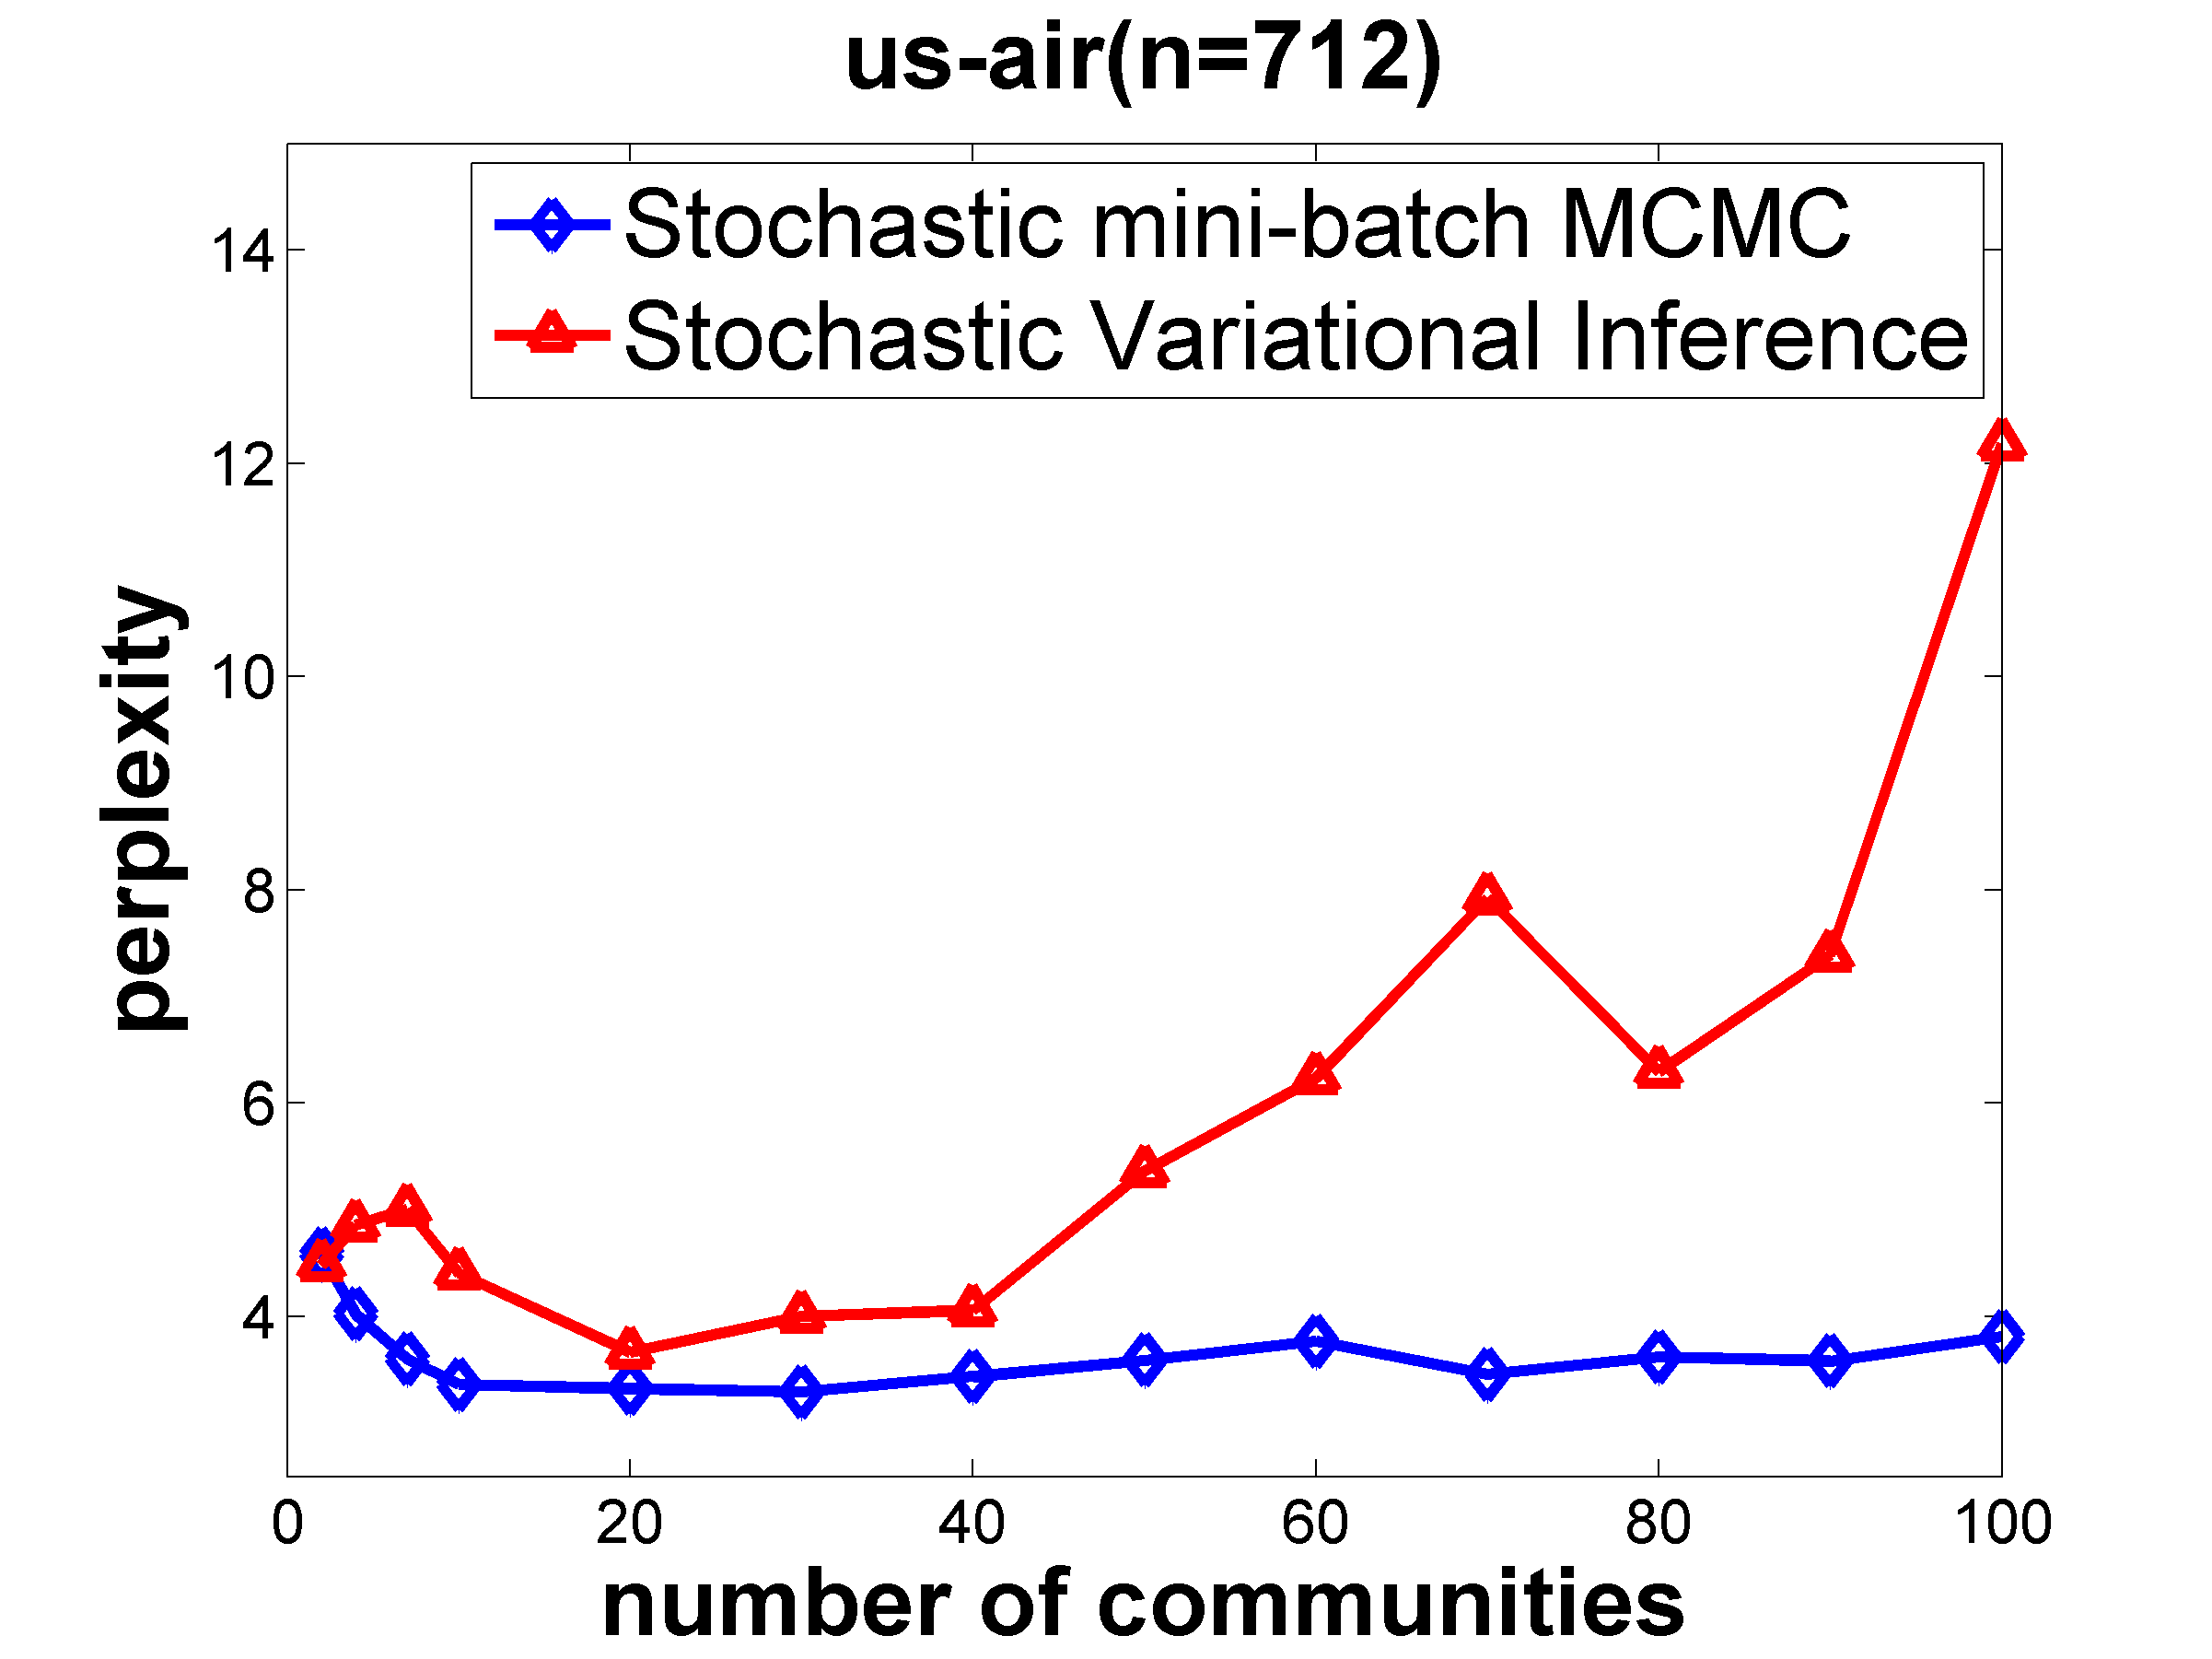
\includegraphics[height=2cm]{3rd_usair}
  \end{subfigure}\\
\caption{SG-MCMC vs SVI}\label{fig:1}
\end{figure}

\begin{itemize}
\item Submitted to AISTATS 2015
\item Extended version(with 1.8B edges) may be submitted to KDD 2015
\end{itemize}
\end{frame}
%%%%%%%%%%%%%%%%%%%%%%%%%%%%%%%%%  Slide 1.5  %%%%%%%%%%%%%%%%%%%%%%%%%%%%%%%%%%%%%%%%%%%
\begin{frame}{Memory Efficient Bayesian Deep Factored Mixed Membership Models}
\begin{figure}
  \begin{center}
  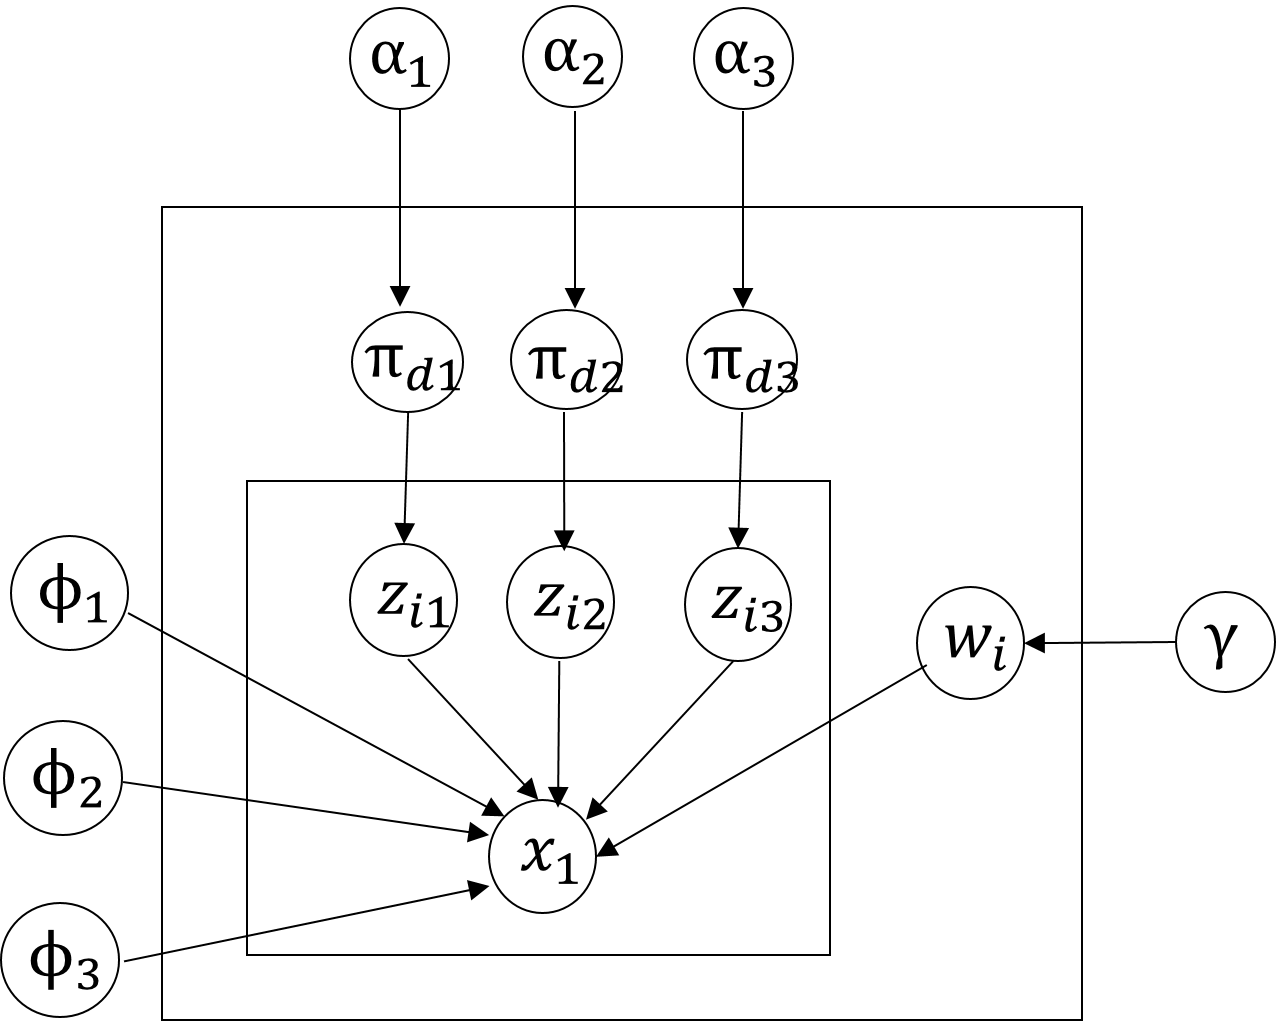
\includegraphics[scale=0.17]{lda.png}
  \caption{3-layer factored LDA}
  \label{fig:distributed}
  \end{center}
\end{figure}

\begin{itemize}
\item[] For each document $d$,
    \begin{itemize}
        \item[] for each layer $l$
        \item[] ~~~~ draw (sub)topic distribution $\pi_{dl}$
    \end{itemize}
    \begin{itemize}
        \item[] for each word $i$
        \item[] ~~~~ draw (sub)topic $z_{il}$ for $l\in \{1,..,L\}$
        \item[] ~~~~ draw word $x_i$ from convex combination of $\{\phi_l\}$
        \end{itemize}
\end{itemize}


\end{frame}

\begin{frame}{Memory Efficient Bayesian Deep Factored Mixed Membership Models(cont.)}
Some benefits:
\begin{itemize}
\item Suppose 3-layer model, each layer has $L_1,L_2,L_3$ components, this can represent $\prod_{i=1}^{3}L_i$ mixtures (exponential).
\item Less parameters comparing to shallow models.
\item Less memory. (becomes very obvious once we have $k$ equals to hundreds of thousand, uses logarithm amount of space comparing to original model)
\item Some hierarchical structures
\end{itemize}

Learning:
\begin{itemize}
\item (Stochastic) variational inference, fixed point iteration, L-BFGS
\item Or propose better inference
\end{itemize}
Progress:\\
~~~~~Coding, Debugging.... (also need to include deep factored MMSB)
\end{frame}

%%%%%%%%%%%%%%%%%%%%%%%%%%%%%%%%%  Slide 1  %%%%%%%%%%%%%%%%%%%%%%%%%%%%%%%%%%%%%%%%%%%

%%%%%%%%%%%%%%%%%%%%%%%%%%%%%%%%%%%%%  slide 2  %%%%%%%%%%%%%%%%%%%%%%%%%%%%%%%%%%%%%%%%%
\begin{frame}{Parallel Stochastic Variational Inference for Bayesian
Tensor Factorization}

\begin{figure}
  \begin{subfigure}[b]{.3\linewidth}
    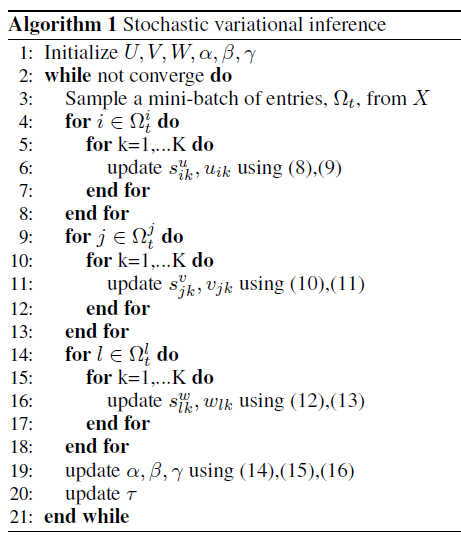
\includegraphics[height=4cm]{svi.png}
  \end{subfigure}
  \begin{subfigure}[b]{.65\linewidth}
    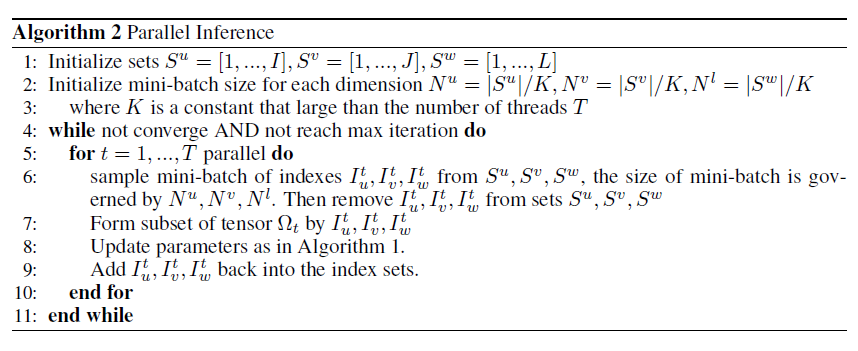
\includegraphics[height=4cm]{svi2.png}
  \end{subfigure}
\end{figure}
Extension: distributed settings
\end{frame}

\begin{frame}{Learning from Ordinal Data}
\begin{itemize}
\item hmm.. this is a hard problem...
\item need a simple, elegant solution....
\item Working hard on experiments, will tell you more about this.
\end{itemize}

\end{frame}

%%%%%%%%%%%%%%%%%%%%%%%%%%%%%%%%%  Slide 3  %%%%%%%%%%%%%%%%%%%%%%%%%%%%%%%%%%%%%%%%%%%
\begin{frame}{Plan for winter}
\begin{itemize}
    \item Coding :)
    \item Debugging :(
    \item Getting results :)
\end{itemize}

\end{frame}


%%%%%%%%%%

\end{document}
